\documentclass[
	% -- opções da classe memoir --
	12pt,				% tamanho da fonte
	openright,			% capítulos começam em pág ímpar (insere página vazia caso preciso)
	twoside,			% para impressão em recto e verso. Oposto a oneside
	a4paper,			% tamanho do papel.
	% -- opções da classe abntex2 --
	%chapter=TITLE,		% títulos de capítulos convertidos em letras maiúsculas
	%section=TITLE,		% títulos de seções convertidos em letras maiúsculas
	%subsection=TITLE,	% títulos de subseções convertidos em letras maiúsculas
	%subsubsection=TITLE,% títulos de subsubseções convertidos em letras maiúsculas
	% -- opções do pacote babel --
	english,			% idioma adicional para hifenização
	french,				% idioma adicional para hifenização
	spanish,			% idioma adicional para hifenização
	brazil,				% o último idioma é o principal do documento
	]{abntex2}


% ---
% PACOTES
% ---

% ---
% Pacotes fundamentais
% ---
\usepackage{lmodern}			% Usa a fonte Latin Modern
\usepackage[T1]{fontenc}		% Selecao de codigos de fonte.
\usepackage[utf8]{inputenc}		% Codificacao do documento (conversão automática dos acentos)
\usepackage{indentfirst}		% Indenta o primeiro parágrafo de cada seção.
\usepackage{color}				% Controle das cores
\usepackage{graphicx}			% Inclusão de gráficos
\usepackage{microtype} 			% para melhorias de justificação
% ---

% ---
% Pacotes adicionais, usados no anexo do modelo de folha de identificação
% ---
\usepackage{multicol}
\usepackage{multirow}
% ---
\usepackage{amsmath}
\usepackage{amssymb}
\usepackage{array}
\usepackage{graphicx}

\begin{document}
	\begin{equation}{\displaystyle}
	  \begin{cases}
	  \frac{dx}{dt}=\sigma(y-x)\\
	  \frac{dy}{dt}=x(\rho-z)-y\\
	  \frac{dz}{dt}=xy-\beta z
	  \end{cases}
	\end{equation}\\

	\begin{equation}
	  F(x)=\frac{1}{2\pi}\int_{\infty}^{-\infty}s(x)e^{-ikx}\mathrm{d}x
	\end{equation}

\newpage

    \begin{table}[htb]
      \begin{center}
      	\caption{Propriedades das substâncias halogênias}
      	\begin{tabular}{cccc}
      	\textbf{Substância} & \textbf{Aparência na CNTP} & \textbf{Ponto de fusão (°C)} & \textbf{Ponde de ebulição (°C)}\\
      	\hline
      	$F_2$ & Gás amarelo claro & -219 & -188\\
      	\hline
      	$Cl_2$ & Gás verde claro & -101 & -34\\
      	\hline
      	$Br_2$ & Líquido castanho oleoso & -7 & -60\\
      	\hline
      	$I_2$ & Sólido preto-arroxeado lustroso & +114 & +185
        \end{tabular}
      \end{center}
    \end{table}

    \begin{table}[htb]

    	\IBGEtab{%
    		\caption{Propriedades das substâncias halogênias.}%
    		\label{tab:ibge}
    	}{%
    		\begin{tabular}{cccc}
    			\toprule
    			Substância & Aparência na CNTP & Ponto de fusão (°C) & Ponto de ebulição (°C)\\
    			\midrule \midrule
    			$F_2$ & Gás amarelo claro & -219 & -188 \\
    			\midrule
    			$Cl_2$ & Gás verde claro & -101 & -34 \\
    			\midrule
    			$Br_2$ & Líquido castanho oleoso & -7 & -60 \\
    			\midrule
    			$I_2$ & Sólido preto-arroxeado lustroso & +114 & +185 \\
    			\bottomrule
    		\end{tabular}%
    	}{%
    		\fonte{http://www.quimica.ufpr.br/paginas/marcio-peres/wp-content/uploads/sites/6/2018/06/Familia-dos-Halogenios-1.pdf}%
    	}
    \end{table}

\newpage

\begin{figure}
	\centering
	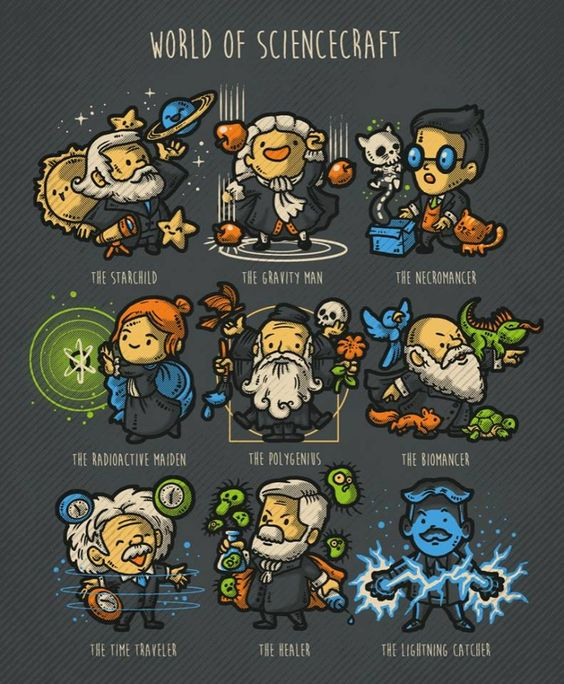
\includegraphics[width=0.85\linewidth, height=0.65\linewidth]{mestres/mestres}
	\caption{}
	\label{fig:mestres}
\end{figure}

\end{document}
%%% Local Variables:
%%% mode: latex
%%% TeX-master: t
%%% End:
